\section{Fixed NPF regime}
In the fixed NPF regime, we forcefully \emph{turn-off} feature learning, i.e., we let the feature gradient $\psi^{\phi}_{x,\Theta}=0$. In order to do this, we hold the gates and hence the NPFs in a separate gating network parameterised by $\Tg\inrdnet$, and the NPVs in a different network called value network parameterised by $\Theta\inrdnet$ (see \Cref{tb:dgn}). By letting the parameters of the gating network non-trainable, i.e., $\Tg_0=\Tg_t,\forall t\geq 0$ we can force $\psi^{\phi}_{x,\Theta}$ to be $0$. Thus, the gates are copied from the gating network onto the value network as shown in the cartoon on the right in \Cref{tb:dgn}.
\begin{table}[h] 
\begin{minipage}{0.75\columnwidth}
\resizebox{\columnwidth}{!}{
\begin{tabular}{|l|l|l|}\hline
Layer& Gating Network (NPF)&Value Network (NPV)\\\hline 
Input & $z_{x,\Tg_t}(0)=x$ &$z_{x,\Theta_t}(0)=x$ \\\hline
Activation & $q_{x,\Tg_t}(l)={\Tg_t(l)}^\top z_{x,\Tg_t}(l-1)$& $q_{x,\Theta_t}(l)={\Theta_t(l)}^\top z_{x,\Theta_t}(l-1)$\\\hline
Hidden &$z_{x,\Tg_t}(l)=\chi^G\left(q_{x,\Tg_t}(l)\right)$& $z_{x,\Theta_t}(l)=q_{x,\Theta_t}(l)\odot G_{x,\Tg_t}(l)$ \\\hline
Output & None &$\hat{y}_t(x)={\Theta_t(d)}^\top z_{x,\Theta_t}(d-1)$\\\hline
\multicolumn{3}{|l|}{Gating Values:\quad$ G_{x,\Tg_t}(l)= \gamma_{r}\left(q_{x,\Tg_t}(l)\right)\quad$or $G_{x,\Tg_t}(l)= \gamma_{sr}\left(q_{x,\Tg_t}(l)\right)$}\\\hline
\end{tabular}
}
\end{minipage}
\begin{minipage}{0.24\columnwidth}
\resizebox{\columnwidth}{!}{
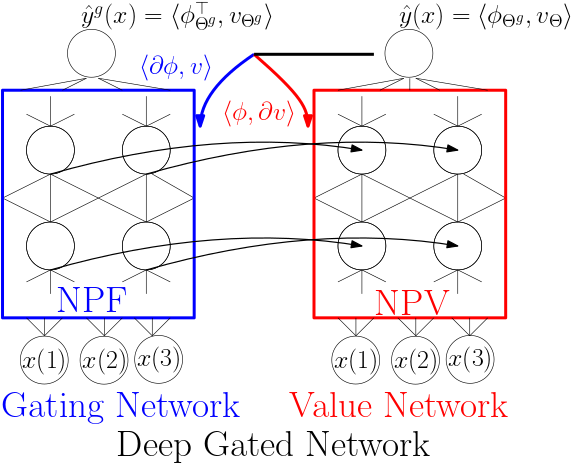
\includegraphics[scale=0.5]{figs/nntwin-blck.png}
}
\end{minipage}
\caption{Setup to learn with fixed NPFs.}
\label{tb:dgn}
\end{table}
\begin{wrapfigure}{h}{0.3\textwidth}
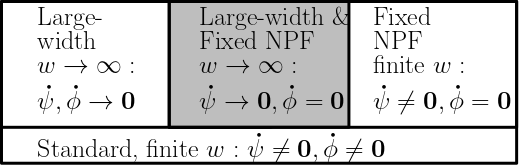
\includegraphics[scale=0.25]{figs/regime.png}
\caption{\label{fig:regime} Regimes.}
\end{wrapfigure}
A comparison of the GD dynamics across the three regimes namely i) the standard regime, wherein, width is finite, and the NPFs are learnt, ii) the `large-width' regime, in which the NPFs, NTFs do not deviate much from initialisation and iii) the fixed NPF regime are given in \Cref{tb:dynamics}. Note that if we let $w\ra\infty$ in the fixed NPF regime, can have a regime which is both `large-width' as well as fixed NPF (see middle region in \Cref{fig:regime}). Further, in the fixed NPF regime, $K_{\Theta}=K^v_{\Theta}$.
\FloatBarrier
\begin{table}[h]\centering
\resizebox{\columnwidth}{!}{
\begin{tabular}{| l | l | l |}\hline
Finite $w$ with NPF learning (standard) & Large-Width & Fixed NPF\\\hline
$\dot{\Theta}_t=-\sum_{s=1}^n (\psi^v_{x_s,t}+\psi^{\phi}_{x_s,t})e_t(s)$ &$\dot{\Theta}_t\ra 0$ &$\dot{\Theta}_t=-\sum_{s=1}^n \psi^v_{x,t}e_t(s)$ \\\hline
$\dot{\phi}_{x_s,t}(p)=x(\I_0(p))\sum_{\theta\in\Theta}\partial_{\theta}A_t(x_s,p)\dot{\theta}_t$ &$\dot{\phi}_{x_s,t}(p)\ra 0$ &$\dot{\phi}_{x_s,t}(p)=0$\\\hline
$\dot{v}_t(p)=\sum_{\theta\in\Theta}\partial_{\theta}v_t(p)\dot{\theta}_t$ &$\dot{v}_t(p)\ra 0$ &$\dot{v}_t(p)=\sum_{\theta\in\Theta}\partial_{\theta}v_t(p)\dot{\theta}_t$\\\hline
$\dot{e}_t=-(K^v_t+K^{\phi}_t+K^{cross}_{t})e_t$ &$\dot{e}_t=-K^{(d)}e_t$ &$\dot{e}_t=-K^v_te_t$\\\hline
\end{tabular}
}
\caption{Dynamics in various regimes. Here $p\in[P], s\in[n]$.}
\label{tb:dynamics}
\end{table}
\begin{assumption}[Independent Initialisation]\label{assmp:main}
(i) $\Theta_0\inrdnet$ is statistically independent of NPFs, (ii) $\Theta_0$ are sampled i.i.d from a distribution such that for any $\theta_0\in\Theta_0$,  we have $\E{\theta_0}=0$, and  $\E{\theta^2_0}=\sigma^2$, and $\E{\theta^4_0}={\sigma'}^2$.
\end{assumption}
\begin{theorem}[\textbf{Main Result}]\label{th:main} Let $H_{\Tg_0}=\Phi^\top_{\Tg_0}\Phi_{\Tg_0}$ be the neural path kernel (NPK) matrix , then under \Cref{assmp:main}, we have:\\
(i) $\E{K_{\Theta_0}}=d\sigma^{2(d-1)} H_{\Tg_0}.$

(ii) In addition, if ${4d}/{w^2}<1$, then $Var\left[K_0\right]\leq O\left(d^2_{in}\sigma^{4(d-1)}\max\{d^2w^{2(d-2)+1}, d^3w^{2(d-2)}\}\right)$.
\end{theorem}
\textbf{Remark on\Cref{assmp:main} :} This is known as the \emph{independent initialisation} case, because, the NPVs $v_{\Theta_0}$ and NPFs $\phi_{x_s,\Tg_0},s\in[n]$ are statistically independent at initialisation. Note that, in a standard DNN with ReLU activations, at initialisation, NPFs and NPV are derived from the same $\Theta_0$, i.e., $\Tg_0=\Theta_0$; we call this case as the \emph{dependent initialisation} which does not satisfy \Cref{assmp:main}. In the case of \emph{dependent initialisation}, $K_{\Theta_0}\ra K^{(d)}$, where $K^{(d)}$ can be calculated by letting $\chi=\chi_{r}$ in \eqref{eq:ntkold} (note that in the fixed NPF regime feature gradient is $0$, and hence $\dot{\gamma}=0$).

\textbf{Remark on \Cref{th:main}:} This result says that in the fixed NPF regime, in the limit of infinite width, at random initialisation as per \Cref{assmp:main}, the NTK $K_{\Theta_0}$ is equal to the NPK $H_{\Tg_0}$ times a scaling constant. From pervious results, \cite{arora2019exact,cao2019generalization}, if follows that as $w\ra\infty$, the optimisation and generalisation properties of the fixed NPF learner can be tied down to $H_{\Tg_0}$. \Cref{th:main} can be applied in the following two interesting scenarios:\\
$1.$ Learning with random fixed NPFs. Here, we choose $\Tg_0$ according to \Cref{assmp:main}-(ii) and statistically independent of $\Theta_0$. The learning problem in this case is $\hat{y}_{\Theta_t}(x)=\ip{\phi_{x,\Tg_0},v_{\Theta_t}}$.\\
$2.$ Learning with fixed NPFs from pre-trained networks. Here, we copy the weights of a pre-trained network into $\Tg_0$, and then start with a random $\Theta_0$ as \Cref{assmp:main}, i.e., we retain the NPFs and then reset the NPVs to relearn them from scratch. \Cref{th:main} states that a network trained this way will generalise as well as its NPK.

Before we proceed to discuss the two scenarios, we will look at the structure of NPK matrix.
\subsection{Hadamard Structure of NPK}
\begin{definition}[Correlation of Sub-Networks]\label{def:lambda}
Let $\tau_{\Theta}(s,s',l)\stackrel{def}=\sum_{i=1}^w G_{x_s,\Theta}(l,i)G_{x_{s'},\Theta}(l,i)$ be the number of activations that are \emph{on} for both inputs $s,s'\in[n]$ in layer $l$. Let $p\rsa i$ denote the fact that path $p$ passes through input node $i\in[d_{in}]$, then define $\Lambda_{\Theta}(s,s')\stackrel{def}{=}\sum_{p\rsa i} A_{\Theta}(x_s,p) A_{\Theta}(x_{s'},p)$, $\forall s,s'\in[n]$, any $i\in [d_{in}]$.
\end{definition}
In the \Cref{def:lambda} above, $\Lambda_{\Theta}\in\R^{n\times n}$ is the correlation matrix of the active sub-networks (consisting of the activations that are \emph{on}) of different input pairs $s,s'\in[n]$. Note that the definition of $\Lambda_{\Theta}$ is not dependent on the choice of input node $i$, because, the terms inside the summation depend only on the path followed from the first layer onwards and excludes the input node.

\begin{lemma}\label{lm:npk}
It follows that:

i) $\Lambda_{\Theta}(s,s')=\Pi_{l=1}^{d-1}\tau_{\Theta}(s,s',l)$.

ii) $H_{\Theta}= \Sigma\odot\Lambda_{\Theta}$, where $\odot$ stands for the Hadamard product, and $\Sigma \in \R^{n\times n}$ is the input Gram matrix.
\end{lemma}


We will now discuss about an interesting application of \Cref{th:main} to the problem of learning with fixed random NPFs.
\subsection{Optimisation with fixed random NPFs at random initialisation: Role of Depth}
Consider the case of independent initialisation, with $w\ra\infty$. Here, $K_{\Theta_0}\ra d\sigma^{(d-1)}H_{\Tg_0}=d(\Sigma)\odot(\sigma^{2(d-1)}\Lambda_{\Tg_0})$. Let us look at the diagonal and non-diagonal entries of $\sigma^{2(d-1)}\Lambda_0$, when $\Tg_0$ is initialised according to \Cref{assmp:main}-(ii) for $\sigma=\sqrt{\frac2w}$.\\
$\bullet$ \emph{Diagonal terms:} $\sqrt{\frac2w}\Lambda_{\Tg_0}(s,s)=2^{(d-1)}\Pi_{l=1}^{(d-1)}\frac{\tau_{\Tg_0}(s,s',l)}w$. Note that as $w\ra\infty$, $\frac{\tau_{\Tg_0}(s,s',l)}w\ra\frac12$, and hence $\sqrt{\frac2w}\Lambda_o(s,s)\ra 1$.\\
$\bullet$ \emph{Non-Diagonal terms:} As $w\ra\infty$, $\sqrt{\frac2w}\Lambda_{\Tg_0}(s,s')=2^{(d-1)}\Pi_{l=1}^{(d-1)}\frac{\tau_{\Tg_0}(s,s',l)}w\ra \Pi_{l=1}^{(d-1)}\mu_l(s,s')$, where $\mu_l(s,s')\in(0,1)$ is the fractional overlap between \emph{on} activation in layer $l$ for inputs $s,s'\in[n]$. Thus as depth increases the non-diagonal terms get suppressed by a factor $\Pi_{l}^{(d-1)}\mu_{l}(s,s')$.

When optimising with fixed NPFs, when the width is finite, increasing depth till a point helps in training due to the suppression of the non-diagonal terms of $H_{\Tg_0}$. Increasing depth beyond a point hurts, because, the variance term has a depth dependence, due to which, the entires of $K_{\Theta_0}$ deviate from their expected values.
\begin{comment}
\begin{table}[h]
\centering
\resizebox{\columnwidth}{!}{
\begin{tabular}{|c|c|c|c|}\hline
		&Gate&Activation&$\dot{\chi}$\\\hline
Prior&$G_R(q)=\mathbbm{1}_{\{q>0\}}$& $\begin{aligned}\chi_{R}(q)&=q\cdot\mathbbm{1}_{\{q>0\}}\\ \chi_{SP}(q)&=\frac{1}{\beta}\log(1+\exp(\beta q))\end{aligned}$&$\begin{aligned}\dot{\chi_{R}}(q)&: \text{Heaviside step function} \\ \dot{\chi}_{SP}(q)&=\frac{1}{1+\exp(-\beta q)}\end{aligned}$ \\\hline
Ours &$G_{SR}(q)=\frac{1}{1+\exp(-\beta q)}$ &$\chi_{SR}(q)=q\cdot G_{SR}(q)$& $\dot{\chi}_{SR}(q)=\dot{\chi}_{SP}(q)+\underbrace{\dot{G}_{SR}(q)}_{\text{Gate Dynamics}}$\\\hline
\end{tabular}
}
\caption{A comparison of prior work and our paper. Here subscripts $R$, $SR$ and $SP$ stand for ReLU, soft-ReLU and softplus respectively.}
\label{tb:compare}
\end{table}
\begin{table}[h]
\centering
\resizebox{\columnwidth}{!}{
\begin{tabular}{|c|c|c|c|c|}\hline
		&Output&NTF&$NTK$ &$\dot{\Sigma}^{(l+1)}(s,s')$\\\hline
Prior&\shortstack{$\hat{y}_{\Theta}(x)$\\layer-by-layer} &$\psi_{x,\Theta}=\left(\partial_{\theta}\hat{y}_{\Theta}(x),\theta\in\Theta\right)$& $K_{\Theta}(x,x')=\ip{\psi_{x,\Theta},\psi_{x',\Theta}}$ & $\dot{\chi}_{SP}(q)\dot{\chi}_{SP}(q')$ \\\hline
Ours& $\hat{y}_{\Theta}(x)=\ip{\phi_{x,\Theta},v_{\Theta}}$ & $\begin{aligned}\psi_{x,\Theta}&=\psi^v_{x,\Theta}+\psi^{\phi}_{x,\Theta}\\\psi^v_{x,\Theta}&=\left(\ip{\phi_{x,\Theta}, \partial_{\theta} v_{\Theta}},\theta\in\Theta\right) \\ \psi^{\phi}_{x,\Theta}&=\left(\ip{\partial_{\theta}\phi_{x,\Theta}, v_{\Theta}},\theta\in\Theta\right)\end{aligned}$ &$\begin{aligned} K_{\Theta}(x,x')=\langle \psi^v_{x,\Theta}+\psi^{\phi}_{x,\Theta},\\ \psi^v_{x',\Theta}+\psi^{\phi}_{x',\Theta}\rangle\end{aligned}$ & $\begin{aligned}\left(\dot{\chi}_{SP}(q)+\dot{G}_{SR}(q)\right)\cdot\\\left(\dot{\chi}_{SP}(q')+\dot{G}_{SR}(q')\right)\end{aligned}$ \\\hline

\end{tabular}
}
\caption{A comparison of prior work and our paper. Here subscripts $R$, $SR$ and $SP$ stand for ReLU, soft-ReLU and softplus respectively.}
\label{tb:compare}
\end{table}
\end{comment}
%$\begin{aligned}&\text{Learning}\\ &\text{Regime} \end{aligned}$ 